\documentclass{ximera}

\outcome{Understand how the derivative of an inverse function relates to the original derivative.}

%\usepackage{todonotes}

\newcommand{\todo}{}

\usepackage{tkz-euclide}
\tikzset{>=stealth} %% cool arrow head
\tikzset{shorten <>/.style={ shorten >=#1, shorten <=#1 } } %% allows shorter vectors

\usepackage{tkz-tab}  %% sign charts
\usetikzlibrary{decorations.pathreplacing} 

\usetikzlibrary{backgrounds} %% for boxes around graphs
\usetikzlibrary{shapes,positioning}  %% Clouds and stars
\usetikzlibrary{matrix} %% for matrix
\usepgfplotslibrary{polar} %% for polar plots
\usetkzobj{all}
\usepackage[makeroom]{cancel} %% for strike outs
%\usepackage{mathtools} %% for pretty underbrace % Breaks Ximera
\usepackage{multicol}

\usepackage{polynom}



\usepackage[many]{tcolorbox}  %% for titled boxes
\newtcolorbox{xbox}[1]{%
    tikznode boxed title,
    enhanced,
    arc=0mm,
    interior style={white},
    attach boxed title to top center= {yshift=-\tcboxedtitleheight/2},
    fonttitle=\bfseries,
    colbacktitle=white,coltitle=black,
    boxed title style={size=normal,colframe=white,boxrule=0pt},
    title={#1}}


\usepackage{array}
\setlength{\extrarowheight}{+.1cm}   
\newdimen\digitwidth
\settowidth\digitwidth{9}
\def\divrule#1#2{
\noalign{\moveright#1\digitwidth
\vbox{\hrule width#2\digitwidth}}}





\newcommand{\RR}{\mathbb R}
\newcommand{\R}{\mathbb R}
\newcommand{\N}{\mathbb N}
\newcommand{\Z}{\mathbb Z}

%\renewcommand{\d}{\,d\!}
\renewcommand{\d}{\mathop{}\!d}
\newcommand{\dd}[2][]{\frac{\d #1}{\d #2}}
\newcommand{\pp}[2][]{\frac{\partial #1}{\partial #2}}
\renewcommand{\l}{\ell}
\newcommand{\ddx}{\frac{d}{\d x}}
\newcommand{\ddt}{\frac{d}{\d t}}

\newcommand{\zeroOverZero}{\ensuremath{\boldsymbol{\tfrac{0}{0}}}}
\newcommand{\inftyOverInfty}{\ensuremath{\boldsymbol{\tfrac{\infty}{\infty}}}}
\newcommand{\zeroOverInfty}{\ensuremath{\boldsymbol{\tfrac{0}{\infty}}}}
\newcommand{\zeroTimesInfty}{\ensuremath{\small\boldsymbol{0\cdot \infty}}}
\newcommand{\inftyMinusInfty}{\ensuremath{\small\boldsymbol{\infty - \infty}}}
\newcommand{\oneToInfty}{\ensuremath{\boldsymbol{1^\infty}}}
\newcommand{\zeroToZero}{\ensuremath{\boldsymbol{0^0}}}
\newcommand{\inftyToZero}{\ensuremath{\boldsymbol{\infty^0}}}



\newcommand{\numOverZero}{\ensuremath{\boldsymbol{\tfrac{\#}{0}}}}
\newcommand{\dfn}{\textbf}
%\newcommand{\unit}{\,\mathrm}
\newcommand{\unit}{\mathop{}\!\mathrm}
\newcommand{\eval}[1]{\bigg[ #1 \bigg]}
\newcommand{\seq}[1]{\left( #1 \right)}
\renewcommand{\epsilon}{\varepsilon}
\renewcommand{\iff}{\Leftrightarrow}

\DeclareMathOperator{\arccot}{arccot}
\DeclareMathOperator{\arcsec}{arcsec}
\DeclareMathOperator{\arccsc}{arccsc}
\DeclareMathOperator{\si}{Si}
\DeclareMathOperator{\proj}{proj}
\DeclareMathOperator{\scal}{scal}


\newcommand{\tightoverset}[2]{% for arrow vec
  \mathop{#2}\limits^{\vbox to -.5ex{\kern-0.75ex\hbox{$#1$}\vss}}}
\newcommand{\arrowvec}[1]{\tightoverset{\scriptstyle\rightharpoonup}{#1}}
\renewcommand{\vec}{\mathbf}
\newcommand{\veci}{\vec{i}}
\newcommand{\vecj}{\vec{j}}
\newcommand{\veck}{\vec{k}}
\newcommand{\vecl}{\boldsymbol{\l}}

\newcommand{\dotp}{\bullet}
\newcommand{\cross}{\boldsymbol\times}
\newcommand{\grad}{\boldsymbol\nabla}
\newcommand{\divergence}{\grad\dotp}
\newcommand{\curl}{\grad\cross}
%\DeclareMathOperator{\divergence}{divergence}
%\DeclareMathOperator{\curl}[1]{\grad\cross #1}


\colorlet{textColor}{black} 
\colorlet{background}{white}
\colorlet{penColor}{blue!50!black} % Color of a curve in a plot
\colorlet{penColor2}{red!50!black}% Color of a curve in a plot
\colorlet{penColor3}{red!50!blue} % Color of a curve in a plot
\colorlet{penColor4}{green!50!black} % Color of a curve in a plot
\colorlet{penColor5}{orange!80!black} % Color of a curve in a plot
\colorlet{fill1}{penColor!20} % Color of fill in a plot
\colorlet{fill2}{penColor2!20} % Color of fill in a plot
\colorlet{fillp}{fill1} % Color of positive area
\colorlet{filln}{penColor2!20} % Color of negative area
\colorlet{fill3}{penColor3!20} % Fill
\colorlet{fill4}{penColor4!20} % Fill
\colorlet{fill5}{penColor5!20} % Fill
\colorlet{gridColor}{gray!50} % Color of grid in a plot

\newcommand{\surfaceColor}{violet}
\newcommand{\surfaceColorTwo}{redyellow}
\newcommand{\sliceColor}{greenyellow}




\pgfmathdeclarefunction{gauss}{2}{% gives gaussian
  \pgfmathparse{1/(#2*sqrt(2*pi))*exp(-((x-#1)^2)/(2*#2^2))}%
}


%%%%%%%%%%%%%
%% Vectors
%%%%%%%%%%%%%

%% Simple horiz vectors
\renewcommand{\vector}[1]{\left\langle #1\right\rangle}


%% %% Complex Horiz Vectors with angle brackets
%% \makeatletter
%% \renewcommand{\vector}[2][ , ]{\left\langle%
%%   \def\nextitem{\def\nextitem{#1}}%
%%   \@for \el:=#2\do{\nextitem\el}\right\rangle%
%% }
%% \makeatother

%% %% Vertical Vectors
%% \def\vector#1{\begin{bmatrix}\vecListA#1,,\end{bmatrix}}
%% \def\vecListA#1,{\if,#1,\else #1\cr \expandafter \vecListA \fi}

%%%%%%%%%%%%%
%% End of vectors
%%%%%%%%%%%%%

%\newcommand{\fullwidth}{}
%\newcommand{\normalwidth}{}



%% makes a snazzy t-chart for evaluating functions
%\newenvironment{tchart}{\rowcolors{2}{}{background!90!textColor}\array}{\endarray}

%%This is to help with formatting on future title pages.
\newenvironment{sectionOutcomes}{}{} 



%% Flowchart stuff
%\tikzstyle{startstop} = [rectangle, rounded corners, minimum width=3cm, minimum height=1cm,text centered, draw=black]
%\tikzstyle{question} = [rectangle, minimum width=3cm, minimum height=1cm, text centered, draw=black]
%\tikzstyle{decision} = [trapezium, trapezium left angle=70, trapezium right angle=110, minimum width=3cm, minimum height=1cm, text centered, draw=black]
%\tikzstyle{question} = [rectangle, rounded corners, minimum width=3cm, minimum height=1cm,text centered, draw=black]
%\tikzstyle{process} = [rectangle, minimum width=3cm, minimum height=1cm, text centered, draw=black]
%\tikzstyle{decision} = [trapezium, trapezium left angle=70, trapezium right angle=110, minimum width=3cm, minimum height=1cm, text centered, draw=black]


\title[Dig-In:]{The Inverse Function Theorem}

\begin{document}
\begin{abstract}
  We see the theoretical underpinning of finding the derivative of an
  inverse function at a point.
\end{abstract}
\maketitle

There is one catch to all the explanations given above where we
computed derivatives of inverse functions. To write something like
\[
\ddx(e^y)=e^y\cdot y'
\]
we need to know that the function $y$ \textit{has} a derivative.  The
\textit{Inverse Function Theorem} guarantees this.

\begin{theorem}[Inverse Function Theorem]\index{Inverse Function Theorem}\label{theorem:IFT}
If $f$ is a differentiable function that is one-to-one near $a$ and
$f'(a) \neq 0$, then
\begin{enumerate}
\item $f^{-1}(x)$ is \textbf{defined} for $x$ near $b=f(a)$,
\item $f^{-1}(x)$ is \textbf{differentiable} near $b=f(a)$, 
\item last, but not least:
  \[
  \eval{\ddx f^{-1}(x)}_{x=b}  = \frac{1}{f'(a)}\qquad\text{where}\qquad b = f(a).
  \]
\end{enumerate}
\begin{explanation}
  We will only explain the last result. We know
  \[
  f(f^{-1}(x)) = x,
  \]
  and now we use implicit differentiation (and the chain rule) to
  write
  \begin{align*}
  \ddx f(f^{-1}(x)) &= f'(f^{-1}(x)) (f^{-1})'(x)\\
  &=1.
  \end{align*}
  Solving for $(f^{-1})'(x)$ we see
  \[
  (f^{-1})'(x) = \frac{1}{f'(f^{-1}(x))}.
  \]
  This is what we have written above.
\end{explanation}
\end{theorem}

It is worth giving one more piece of evidence for the formula above,
this time based on increments in function, $\Delta f$, and increments in variable, $\Delta x$. Consider this plot of a function $f$ and its inverse:
\begin{image}
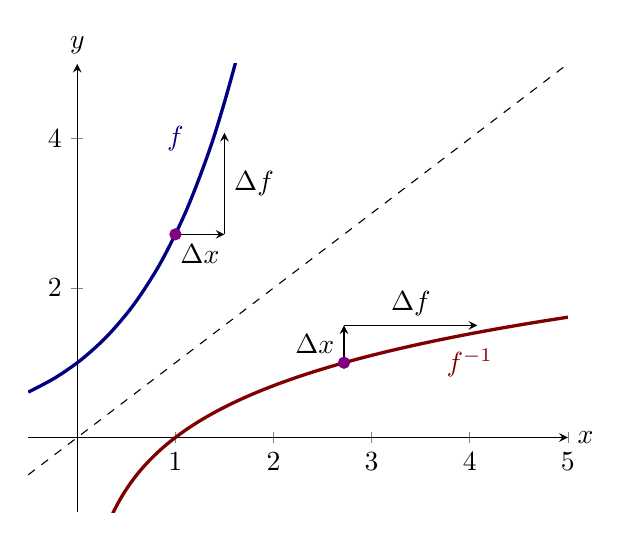
\begin{tikzpicture}
	\begin{axis}[
            xmin=-.5,xmax=5,ymin=-1,ymax=5,
            axis lines=center,
            xlabel=$x$, ylabel=$y$,
            every axis y label/.style={at=(current axis.above origin),anchor=south},
            every axis x label/.style={at=(current axis.right of origin),anchor=west},
          ]        
          \addplot [very thick, penColor, smooth, domain=(-.5:6)] {e^x};
          \addplot [very thick, penColor2, samples=100, smooth, domain=(.002:6)] {ln(x)};
          \addplot [dashed, textColor, domain=(-.5:6)] {x};
          \node at (axis cs:1,4) [penColor] {$f$};
          \node at (axis cs:4,1) [penColor2] {$f^{-1}$};

          \addplot [draw=black,->] plot coordinates {(1,e) (1.5,e)};
	  \addplot [draw=black,->] plot coordinates {(1.5,e) (1.5,1.5*e)};
          \addplot[color=penColor3,fill=penColor3,only marks,mark=*] coordinates{(1,e)};  %% closed hole            
          \node at (axis cs:1.25,e) [below] {$\Delta x$};
          \node at (axis cs:1.5,3.4) [right] {$\Delta f$};

          \addplot [draw=black,->] plot coordinates {(e,1) (e,1.5)};
	  \addplot [draw=black,->] plot coordinates {(e,1.5) (1.5*e,1.5)};
          \addplot[color=penColor3,fill=penColor3,only marks,mark=*] coordinates{(e,1)};  %% closed hole            
          \node at (axis cs:e,1.25) [left] {$\Delta x$};
          \node at (axis cs:3.4,1.5) [above] {$\Delta f$};
        \end{axis}
\end{tikzpicture}
%% \caption{A plot of $e^x$ and $\ln(x)$. Since they are inverse
%%   functions, they are reflections of each other across the line $y=x$.}
%% \label{plot:e^x lnx}
\end{image}
Since the graph of the inverse of a function is the reflection of the graph of the function over
the line $y=x$, we see that the increments are ``switched'' when
reflected. Hence we see that
\[
\dfrac{\Delta f^{-1}}{\Delta{x}} = \dfrac{\Delta x}{\Delta f}=\dfrac{1}{\dfrac{\Delta f}{\Delta x}}.
\]
Taking the limit as $\Delta x$ goes to $0$, we can obtain the expression for the derivative of $f^{-1}$. \\
\[
\dfrac{d f^{-1}}{d{x}} = \dfrac{1}{\dfrac{d f}{d x}}
\]

The inverse function theorem gives us a recipe for computing the
derivatives of inverses of functions at points.

\begin{example}
  Let $f$ be a differentiable function that has an inverse. In the
  table below we give several values for both $f$ and $f'$:
  \[
  \begin{array}{|c|c|c|}\hline
    x & f  & f' \\ \hline \hline
    2 & 0  & 2  \\ \hline
    3 &1  &5 \\ \hline
    4 & 3 & 0  \\ \hline
  \end{array}
  \]
  Compute
  \[
  \ddx f^{-1}(x)\;\text{at $x=1$.}
  \]
  \begin{explanation}
    From the table above we see that
    \[
    1 = f(\answer [given]{3}).
    \]
    Hence, by the inverse function theorem
    \[
    \left(f^{-1}\right)' (1)= \frac{1}{f'(\answer[given]{3})} = \answer[given]{\frac{1}{5}}.
    \]
  \end{explanation}
\end{example}

If one example is good, two are better:

\begin{example}
  Let $f$ be a differentiable function that has an inverse. In the
  table below we give several values for both $f$ and $f'$:
  \[
  \begin{array}{|c|c|c|}\hline
    x & f  & f' \\ \hline \hline
    2 & 0  & 2  \\ \hline
    3 & 1  &5 \\ \hline
    4 & 3 & 0  \\ \hline
  \end{array}
  \]
  Compute
  \[
  \left(f^{-1}\right)'(0)
  \]
  \begin{explanation}
    Note,
    \[
    \left(f^{-1}\right)'(0) = \ddx f^{-1}(x)\;\text{at $x=0$.}
    \]
    From the table above we see that
    \[
    0 = f(\answer[given]{2}).
    \]
    Hence, by the inverse function theorem
    \[
    \left(f^{-1}\right)'(0) = \frac{1}{f'(\answer[given]{2})} = \answer[given]{\frac{1}{2}}.
    \]
  \end{explanation}
\end{example}

Finally, let's see an example where the theorem does not apply.

\begin{example}
  Let $f$ be a differentiable function that has an inverse. In the
  table below we give several values for both $f$ and $f'$:
  \[
  \begin{array}{|c|c|c|}\hline
    x & f  & f' \\ \hline \hline
    2 & 0  & 2  \\ \hline
    3 & 1  & 4 \\ \hline
    4 & 3 & 0  \\ \hline
  \end{array}
  \]
  Compute
  \[
  \eval{\ddx f^{-1}(x)}_{x=3}
  \]
  \begin{explanation}
    From the table above we see that
    \[
    3 = f(\answer[given]{4}).
    \]
    Ah! But here, $f'(\answer[given]{4}) = \answer[given]{0}$, so we have no guarantee that the
    inverse exists near the point $x=3$, but even if it did the inverse would not be differentiable there.
      \end{explanation}
\end{example}


\end{document}
